% ==================================================================
%  §7.4  零值定理、介值定理、最值定理及一致连续性定理
%  源：徐森林、薛春华《数学分析》第二册，印刷页 35-40 (PDF p. 41-46)
%  底本：PaddleOCR-VL-1.6 JSON/MD 识别结果，人工逐字核校与公式精修
%  规范：全西文标点，忠实原文定理、定义、引理、例题、练习题编号与推导
% ==================================================================

\section{零值定理、介值定理、最值定理及一致连续性定理}\label{sec:7.4}

在这一节, 我们将有界闭区间 $[a, b]$ 上连续函数的零值定理, 介值定理, 最值定理及一致连续性定理推广到 $n$ 维 Euclid 空间, 以至拓扑空间.

\begin{theorem}[介值定理]\label{thm:7.4.1}
设 $(X, \mathcal{T})$ 连通, $(\mathbb{R}^{1}, \mathcal{T}_{\rho_{0}}^{1}) = (\mathbb{R}, \mathcal{T}_{\rho_{0}}^{1})$ 为通常的实直线, $f\colon X \to \mathbb{R}^{1}$ 为连续函数, $p, q \in X$, 则 $f$ 达到介于 $f(p)$ 与 $f(q)$ 之间的一切值, 即 $\exists \xi \in X$, s. t.
\[
  f(\xi) = r \in [\min\{f(p), f(q)\}, \max\{f(p), f(q)\}].
\]
\end{theorem}

\begin{proof}
由\cref{thm:7.2.7}(1), $f(X)$ 为 $(\mathbb{R}^{1}, \mathcal{T}_{\rho_{0}}^{1})$ 中的连通集, 即为实直线上的区间 (当 $f$ 为常值函数时缩成一点), 所以 $f$ 达到 $f(p)$ 与 $f(q)$ 之间的一切值.
\end{proof}

\begin{theorem}[零 (根) 值定理]\label{thm:7.4.2}
设 $(X, \mathcal{T})$ 连通, $f\colon X \to \mathbb{R}$ 为连续函数, $p, q \in X$, 如果 $f(p)f(q) \leqslant 0$, 则 $\exists \xi \in X$, s. t. $f(\xi) = 0$.
\end{theorem}

\begin{proof}
因为 $f(p)f(q) \leqslant 0$, 所以 $r = 0 \in [\min\{f(p), f(q)\}, \max\{f(p), f(q)\}]$, 由\cref{thm:7.4.1} (介值定理), $\exists \xi \in X$, s. t. $f(\xi) = 0$.
\end{proof}

\begin{example}[Borsuk-Ulam 定理]\label{ex:7.4.1}
设 $S^{n} = \left\{(x_{1}, x_{2}, \cdots, x_{n+1}) \mid \sum\limits_{i=1}^{n+1} x_{i}^{2} = 1\right\} \subset \mathbb{R}^{n+1}$ 为 $n$ 维单位球面 ($n \in \mathbb{Z}_{+}$), $f\colon S^{n} \to \mathbb{R}^{1}$ 为连续函数. 则 $\exists \xi \in S^{n}$, s. t. $f(\xi) = f(-\xi)$.
\end{example}

\begin{proof}
$\forall p, q \in S^{n}$, 取一个过球心的二维平面, s. t. $e_{1} = p$, $\{e_{1}, e_{2}\}$ 构成该平面的规范正交基, 而 $q$ 也在此平面内 (\cref{fig:7.4.1}). 于是, $q = \cos\theta_{0} e_{1} + \sin\theta_{0} e_{2}$.

显然, $\boldsymbol{\sigma}(t) = \cos t\theta_{0} e_{1} + \sin t\theta_{0} e_{2}$ 为球面 $S^{n}$ 上连接 $p$ 与 $q$ 的一条道路. 因此, $S^{n}$ 是道路连通的, 根据\cref{thm:7.2.5}, $S^{n}$ 是连通的.

\begin{figure}[htbp]
  \centering
  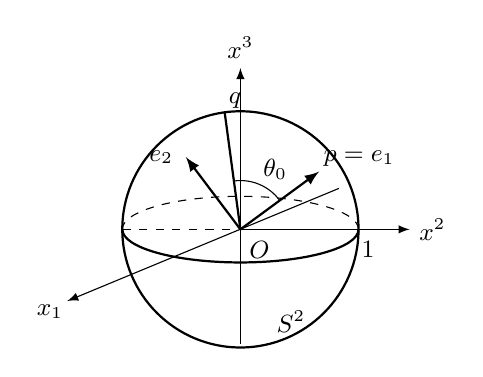
\begin{tikzpicture}[>=latex, scale=1.0]
    % ---- 球面 S^2 ----
    \draw[thick] (0, 0) circle (1.5);
    % 赤道椭圆: 后半虚线、前半实线; 以及过球心的虚线直径
    \draw[dashed] (1.5, 0) arc (0:180:1.5 and 0.42);
    \draw[thick] (1.5, 0) arc (0:-180:1.5 and 0.42);
    \draw[dashed] (-1.5, 0) -- (1.5, 0);
    % ---- 坐标轴 ----
    \draw[->] (0, -1.45) -- (0, 2.05) node[above] {\small $x^{3}$};
    \draw[->] (0, 0) -- (2.15, 0) node[right] {\small $x^{2}$};
    \draw[->] (1.25, 0.52) -- (-2.20, -0.91) node[below left=-2pt] {\small $x_{1}$};
    \node[below=1pt] at (1.62, 0) {\small $1$};
    \node[below right=-2pt] at (0.06, -0.10) {\small $O$};
    % ---- 球面上的点 q, 向径 Oq ----
    \coordinate (q) at (-0.20, 1.487);
    \draw[thick] (0, 0) -- (q);
    \node[above right=-2pt] at (q) {\small $\boldsymbol{q}$};
    % ---- 向量 p = e_1 与 e_2 ----
    \draw[->, thick] (0, 0) -- (36.3:1.24) node[above right=-2pt] {\small $\boldsymbol{p} = \boldsymbol{e}_{1}$};
    \draw[->, thick] (0, 0) -- (127:1.15) node[left=1pt] {\small $\boldsymbol{e}_{2}$};
    % ---- 夹角 theta_0 ----
    \draw (36.3:0.62) arc (36.3:97.7:0.62);
    \node at (60:0.88) {\small $\theta_{0}$};
    % ---- 球面标签 ----
    \node at (0.64, -1.17) {\small $S^{2}$};
  \end{tikzpicture}
  \caption{}\label{fig:7.4.1}
\end{figure}

令
\[
  F(\boldsymbol{x}) = f(\boldsymbol{x}) - f(-\boldsymbol{x}),\quad \boldsymbol{x} = (x_{1}, x_{2}, x_{3}),
\]
则
\[
  \begin{aligned}
    F(\boldsymbol{p})F(-\boldsymbol{p}) &= [f(\boldsymbol{p}) - f(-\boldsymbol{p})][f(-\boldsymbol{p}) - f(\boldsymbol{p})]\\
    &= -[f(\boldsymbol{p}) - f(-\boldsymbol{p})]^{2} \leqslant 0.
  \end{aligned}
\]
根据\cref{thm:7.4.2}, $\exists \xi \in S^{n}$, s. t.
\[
  0 = F(\xi) = f(\xi) - f(-\xi),
\]
即 $f(\xi) = f(-\xi)$.
\end{proof}

\begin{theorem}[最值定理]\label{thm:7.4.3}
设 $(X, \mathcal{T})$ 为紧致 (或可数紧致, 或序列紧致) 空间, $(\mathbb{R}^{1}, \mathcal{T}_{\rho_{0}}^{1})$ 为通常的一维 Euclid 空间, $f\colon X \to \mathbb{R}^{1}$ 为连续函数, 则 $f$ 在 $X$ 上必达到最大值与最小值. 此时, $f(X) = [m, M]$, 其中 $m = \min\limits_{x \in X} f(x)$, $M = \max\limits_{x \in X} f(x)$.
\end{theorem}

\begin{proof}
由\cref{thm:7.3.7}, $f(X)$ 为 $(\mathbb{R}^{1}, \mathcal{T}_{\rho_{0}}^{1})$ 中的紧致 (或可数紧致, 或序列紧致) 子集. 再由\cref{thm:7.3.6}知, $f(X)$ 为 $(\mathbb{R}^{1}, \mathcal{T}_{\rho_{0}}^{1})$ 中的有界闭集. 因此 $\min\limits_{x \in X} f(x)$, $\max\limits_{x \in X} f(x)$ 分别为 $f$ 在 $X$ 上的最小值与最大值.
\end{proof}

\begin{corollary}\label{cor:7.4.1}
设 $(X, \mathcal{T}_{\rho})$ 为列紧度量空间, $(\mathbb{R}^{1}, \mathcal{T}_{\rho_{0}}^{1})$ 为通常的一维 Euclid 空间, $f\colon X \to \mathbb{R}^{1}$ 为连续函数, 则 $f$ 在 $X$ 上必达到最大值与最小值.
\end{corollary}

\begin{proof}
由\cref{thm:7.3.2}, 列紧度量空间 $(X, \mathcal{T}_{\rho})$ 也是可数紧致, 也是序列紧致的, 再根据\cref{thm:7.4.3}, $f$ 在 $X$ 上必达到最大值与最小值.
\end{proof}

\begin{theorem}[Lebesgue 数定理]\label{thm:7.4.4}
设 $(X, \rho)$ 为序列紧致 (或可数紧致, 或列紧, 或紧致) 度量空间, $\mathcal{T}$ 为 $X$ 的一个开覆盖 (即 $X = \bigcup\limits_{I \in \mathcal{T}} I$, $I$ 为 $(X, \mathcal{T}_{\rho})$ 中的开集), 则存在一个正数 $\lambda = \lambda(\mathcal{T})$ 具有性质: 如果 $A \subset X$, 其直径
\[
  d(A) = \operatorname{diam} A = \sup\{\rho(x', x'') \mid x', x'' \in A\} < \lambda = \lambda(\mathcal{T})
\]
时, 必有 $I \in \mathcal{T}$, s. t. $A \subset I$. 我们称 $\lambda = \lambda(\mathcal{T})$ 为开覆盖 $\mathcal{T}$ 的一个 Lebesgue 数.
\end{theorem}

\begin{proof}
完全仿照\extref{定理 2.5.6} 的证明.

(反证) 假设结论不成立, 则 $\forall n \in \mathbb{Z}_{+}$, $\exists A_{n} \subset X$, 它的直径 $d(A_{n}) < \dfrac{1}{n}$, 而不存在 $I \in \mathcal{T}$, s. t. $A_{n} \subset I$. 在每个 $A_{n}$ 中取 $a_{n}$. 根据 $(X, \rho)$ 为序列紧致空间, 存在子列 $\{a_{n_{k}}\}$ 收敛于 $a_{0} \in X$. 因为 $\mathcal{T}$ 为 $(X, \mathcal{T}_{\rho})$ 的一个开覆盖, 故存在 $I_{0} \in \mathcal{T}$, 使得 $a_{0} \in I_{0}$. 因为 $I_{0}$ 为开集, 当 $X \setminus I_{0} \neq \varnothing$ 时, 点 $a_{0}$ 到集合 $X \setminus I_{0}$ 的距离
\[
  d = \rho(a_{0}, X \setminus I_{0}) = \inf\{\rho(a_{0}, x) \mid x \in X \setminus I_{0}\} > 0,
\]
由于 $\lim\limits_{k \to +\infty} a_{n_{k}} = a_{0}$, 所以, $\exists n_{k_{0}}$, s. t. $n_{k_{0}} < \dfrac{2}{d}$ 与 $\rho(a_{0}, a_{n_{k_{0}}}) < \dfrac{d}{2}$. 于是, $\forall x \in A_{n_{k_{0}}}$, 有
\[
  \rho(a_{0}, x) \leqslant \rho(a_{0}, a_{n_{k_{0}}}) + \rho(a_{n_{k_{0}}}, x) < \frac{d}{2} + \frac{1}{n_{k_{0}}} < \frac{d}{2} + \frac{d}{2} = d,
\]
因而, $A_{n_{k_{0}}} \subset I_{0} \in \mathcal{T}$; 当 $X \setminus I_{0} = \varnothing$ 时, $A_{n} \subset X \subset I_{0}$. 这与不存在 $I \in \mathcal{T}$, s. t. $A_{n_{k_{0}}} \subset I$ 相矛盾.
\end{proof}

\begin{theorem}[一致连续性定理]\label{thm:7.4.5}
设 $(X, \rho_{1})$ 为序列紧致 (或可数紧致, 或列紧, 或紧致) 的度量空间, $(Y, \rho_{2})$ 为度量空间, $f\colon X \to Y$ 为连续映射, 则 $f$ 在 $X$ 上一致连续, 即 $\forall \varepsilon > 0$, $\exists \delta > 0$, 当 $x', x'' \in X$, $\rho_{1}(x', x'') < \delta$ 时, 有 $\rho_{2}(f(x'), f(x'')) < \varepsilon$.
\end{theorem}

\begin{proof}[证法 1]
根据\cref{thm:7.3.2}, 只需考虑序列紧致情况.

(反证) 假设 $f$ 在 $X$ 上不一致连续, 则 $\exists \varepsilon_{0} > 0$, $\forall n \in \mathbb{Z}_{+}$, 必有 $x_{n}', x_{n}''$, s. t. $\rho_{1}(x_{n}', x_{n}'') < \dfrac{1}{n}$, 但 $\rho_{2}(f(x_{n}'), f(x_{n}'')) \geqslant \varepsilon_{0}$. 因为 $(X, \mathcal{T}_{\rho_{1}})$ 序列紧致, 故 $\{x_{n}'\}$ 必有收敛子列 $\{x_{n_{k}}'\}$, 记 $\lim\limits_{k \to +\infty} x_{n_{k}}' = x_{0} \in X$. 由于 $\rho_{1}(x_{n}', x_{n}'') < \dfrac{1}{n}$, 故
\[
  0 \leqslant \rho_{1}(x_{n_{k}}'', x_{0}) \leqslant \rho_{1}(x_{n_{k}}'', x_{n_{k}}') + \rho_{1}(x_{n_{k}}', x_{0}) < \frac{1}{n_{k}} + \rho_{1}(x_{n_{k}}', x_{0}) \to 0\ (k \to +\infty),
\]
即
\[
  \lim\limits_{k \to +\infty} \rho_{1}(x_{n_{k}}'', x_{0}) = 0,\quad \lim\limits_{k \to +\infty} x_{n_{k}}'' = x_{0}.
\]
于是, 由 $f$ 为 $X$ 上的连续函数, $\exists K \in \mathbb{Z}_{+}$, 当 $k > K$ 时, 有
\[
  \begin{aligned}
    \varepsilon_{0} &\leqslant \rho_{2}\left(f(\boldsymbol{x}_{n_{k}}'), f(\boldsymbol{x}_{n_{k}}'')\right)\\
    &\leqslant \rho_{2}\left(f(\boldsymbol{x}_{n_{k}}'), f(\boldsymbol{x}_{0})\right) + \rho_{2}\left(f(\boldsymbol{x}_{0}), f(\boldsymbol{x}_{n_{k}}'')\right)\\
    &< \frac{\varepsilon_{0}}{2} + \frac{\varepsilon_{0}}{2} = \varepsilon_{0},
  \end{aligned}
\]
矛盾. 所以, $f$ 在 $X$ 上一致连续. \noqedhere
\end{proof}

\begin{proof}[证法 2]
设 $(X, \mathcal{T}_{\rho_{1}})$ 紧致. $\forall \varepsilon > 0$, 因为 $f$ 在 $X$ 上连续, 故对 $x \in X$, $\exists \delta(x) > 0$, s. t. 当 $x' \in X$, 且 $\rho_{1}(x', x) < \delta(x)$ 时, 有 $\rho_{2}(f(x'), f(x)) < \dfrac{\varepsilon}{2}$.

显然, 开球族 $\mathcal{T} = \left\{B\left(x; \dfrac{\delta(x)}{2}\right) \middle| x \in X\right\}$ 为紧致空间 $(X, \mathcal{T}_{\rho_{1}})$ 的一个开覆盖. 因此, 存在有限子覆盖 $\mathcal{T}_{1} = \left\{B\left(x_{i}; \dfrac{\delta(x_{i})}{2}\right) \middle| i = 1, 2, \cdots, m\right\}$. 令
\[
  \delta = \min\left\{\frac{\delta(x_{i})}{2} \bigg| i = 1, 2, \cdots, m\right\},
\]
则 $\forall x', x'' \in X$, 当 $\rho_{1}(x', x'') < \delta$ 时, 如果 $x' \in B\left(x_{i_{0}}; \dfrac{\delta(x_{i_{0}})}{2}\right)$, 必有 $x', x'' \in B(x_{i_{0}}; \delta(x_{i_{0}}))$, 从而
\[
  \rho_{2}\left(f(x'), f(x'')\right) \leqslant \rho_{2}\left(f(x'), f(x_{i_{0}})\right) + \rho_{2}\left(f(x_{i_{0}}), f(x'')\right) < \frac{\varepsilon}{2} + \frac{\varepsilon}{2} = \varepsilon,
\]
即 $f$ 在 $X$ 上是一致连续的. \noqedhere
\end{proof}

\begin{proof}[证法 3]
设 $(X, \mathcal{T}_{\rho})$ 序列紧致. 在证法 2 中, 由于 $\mathcal{T}_{1} = \{B(x; \delta(x)) \mid x \in X\}$ 为序列紧致集 $X$ 的一个开覆盖. 根据\cref{thm:7.4.4}, 存在 Lebesgue 数 $\lambda(\mathcal{T}_{1}) > 0$. 对于 $\varepsilon > 0$, 取 $\delta = \lambda(\mathcal{T}_{1})$, 则当 $x', x'' \in X$, 且 $\operatorname{diam}\{x', x''\} = \rho(x', x'') < \delta = \lambda(\mathcal{T}_{1})$ 时, 存在 $B(x_{0}; \delta(x_{0})) \in \mathcal{T}_{1}$, 使得 $\{x', x''\} \subseteq B(x_{0}; \delta(x_{0}))$, 从而,
\[
  \rho_{2}\left(f(x'), f(x'')\right) \leqslant \rho_{2}\left(f(x'), f(x_{0})\right) + \rho_{2}\left(f(x_{0}), f(x'')\right) < \frac{\varepsilon}{2} + \frac{\varepsilon}{2} = \varepsilon.
\]
这就证明了 $f$ 在 $X$ 上是一致连续的.
\end{proof}

\begin{theorem}[延拓定理]\label{thm:7.4.6}
设 $(X, \rho_{1})$ 与 $(Y, \rho_{2})$ 为度量空间, $A \subset X$.
\begin{enumerate}
  \item 如果 $\overline{A}$ 为 $(X, \mathcal{T}_{\rho_{1}})$ 的序列紧致 (或可数紧致, 或列紧, 或紧致) 子集, $f\colon \overline{A} \to Y$ 连续, 则 $f$ 在 $\overline{A}$ (当然也在 $A$) 上一致连续.

  \item 如果 $f\colon A \to Y$ 一致连续, $\overline{f(A)}$ 为 $(Y, \rho_{2})$ 的完备子度量空间, 则存在连续映射 $\tilde{f}\colon \overline{A} \to Y$, 使得 $\tilde{f}|A = f|A$, 即 $\tilde{f}$ 为 $f$ 的 (连续) 延拓.
\end{enumerate}
\end{theorem}

\begin{proof}
(1) 由\cref{thm:7.4.5}推得.

(2) $\forall x_{0} \in \overline{A}$, $x_{n} \in A$, $x_{n} \to x_{0}\ (n \to +\infty)$, 必有 $\lim\limits_{n \to +\infty} f(x_{n})$ 存在, 且 $\lim\limits_{n \to +\infty} f(x_{n}) \in \overline{f(A)}$. 事实上, $\forall \varepsilon > 0$, 由于 $f$ 在 $A$ 上一致连续, 所以存在 $\delta > 0$, 当 $\rho_{1}(x', x'') < \delta$ 时, 有 $\rho_{2}(f(x'), f(x'')) < \varepsilon$. 于是, $\exists N \in \mathbb{Z}_{+}$, 当 $n, m > N$ 时, $\rho_{1}(x_{n}, x_{m}) < \delta$, 从而 $\rho_{2}(f(x_{n}), f(x_{m})) < \varepsilon$. 这意味着 $\{f(x_{n})\}$ 为 $\overline{f(A)} \subset Y$ 中的 Cauchy (基本) 点列. 因为 $\overline{f(A)}$ 为 $(Y, \rho_{2})$ 的完备子度量空间, 所以 $\{f(x_{n})\}$ 在 $\overline{f(A)}$ 中必收敛, 即 $\lim\limits_{n \to +\infty} f(x_{n})$ 存在且属于 $\overline{f(A)}$. 再证 $\lim\limits_{n \to +\infty} f(x_{n})$ 与点列 $\{x_{n}\}$, $x_{n} \to x_{0}\ (n \to +\infty)$ 的选取无关. 如果 $y_{n} \in A$, $y_{n} \to x_{0}\ (n \to +\infty)$, 则 $\{z_{n}\} = \{x_{1}, y_{1}, x_{2}, y_{2}, \cdots, x_{n}, y_{n}, \cdots\}$ 也收敛于 $x_{0}$, 所以 $\{f(z_{n})\}$ 也收敛, 且
\[
  \lim_{n \to +\infty} f(x_{n}) = \lim_{n \to +\infty} f(z_{n}) = \lim_{n \to +\infty} f(y_{n}).
\]
由此与归结原则可知, $\lim\limits_{\substack{x \to x_{0} \\ x \in A}} f(x)$ 存在且属于 $\overline{f(A)}$. 我们定义
\[
  \tilde{f}(x_{0}) = \lim_{\substack{x \to x_{0} \\ x \in A}} f(x).
\]
易见, $\tilde{f}$ 为 $\overline{A}$ 上的连续映射, 且 $\tilde{f}|A = f|A$, 即 $\tilde{f}$ 为 $f$ 的 (连续) 延拓.
\end{proof}

作为一致连续的应用, 我们来考虑下面的重要例子.

\begin{example}\label{ex:7.4.2}
设 $X = ([0, 1] \times \{0\}) \cup \left(\left\{0, 1, \dfrac{1}{2}, \cdots, \dfrac{1}{n}, \cdots\right\} \times [0, 1]\right) \subset \mathbb{R}^{2}$, 称它为篦式空间. 则:

(1) 点 $(0, 1)$ 为 $X$ 的形变收缩核, 即存在连续映射 $F\colon X \times [0, 1] \to X$, 使得
\[
  F((x_{1}, x_{2}), 0) = (x_{1}, x_{2}) = \operatorname{Id}_{X}(x_{1}, x_{2}),
\]
\[
  F((x_{1}, x_{2}), 1) = (0, 1) = C_{(0, 1)}(x_{1}, x_{2}),
\]
其中 $\operatorname{Id}_{X}\colon X \to X$ 为 $X$ 上的恒同映射, $C_{(0, 1)}$ 为 $X$ 上的常值映射.

(2) 点 $(0, 1)$ 不为 $X$ 上的强形变收缩核, 即不存在连续映射 $G\colon X \times [0, 1] \to X$
\[
  G((x_{1}, x_{2}), 0) = (x_{1}, x_{2}) = \operatorname{Id}_{X}(x_{1}, x_{2}),
\]
\[
  G((x_{1}, x_{2}), 1) = (0, 1) = C_{(0, 1)}(x_{1}, x_{2}),
\]
\[
  G((0, 1), t) = (0, 1),\quad \forall t \in [0, 1].
\]

(3) 点 $(0, 0)$ 为 $X$ 上的强形变收缩核 (读者自证).
\end{example}

\begin{proof}
(1) 令 $F\colon X \times [0, 1] \to X$,
\[
  F((x_{1}, x_{2}), t) = \begin{cases}
    (x_{1}, (1 - 3t)x_{2}), & 0 \leqslant t \leqslant \dfrac{1}{3},\\[6pt]
    ((2 - 3t)x_{1}, 0), & \dfrac{1}{3} < t \leqslant \dfrac{2}{3},\\[6pt]
    (0, 3t - 2), & \dfrac{2}{3} < t \leqslant 1
  \end{cases}
\]
为所需的形变收缩, 因此, $(0, 1)$ 为 $X$ 的形变收缩核.

(2) (反证) 假设 $(0, 1)$ 为 $X$ 的强形变收缩核, 即存在 (2) 中所述的连续映射 $G\colon X \times [0, 1] \to X$. 因为 $X \times [0, 1]$ 为紧致集, 故必一致连续. 从而对 $\varepsilon_{0} = \dfrac{1}{2}$, $\exists \delta > 0$, 当
\[
  \left\|(x_{1}, x_{2}, t) - (x_{1}', x_{2}', t')\right\| < \delta
\]
时, 有
\[
  \left\|G(x_{1}, x_{2}, t) - G(x_{1}', x_{2}', t')\right\| < \varepsilon_{0} = \frac{1}{2}.
\]
因此, 当 $\left\|(0, 1, t) - \left(\dfrac{1}{n}, 1, t\right)\right\| = \left\|\left(\dfrac{1}{n}, 0, 0\right)\right\| = \dfrac{1}{n} < \delta$ 时,
\[
  \begin{aligned}
    \left\|(0, 1) - G\left(\frac{1}{n}, 1, t\right)\right\| &= \left\|G(0, 1, t) - G\left(\frac{1}{n}, 1, t\right)\right\|\\
    &< \varepsilon_{0} = \frac{1}{2}.
  \end{aligned}
\]
由此得 $G\left(\dfrac{1}{n}, 1, t\right) \in B\left((0, 1); \dfrac{1}{2}\right)$, $\forall t \in [0, 1]$.

于是, $G\left(\dfrac{1}{n}, 1, t\right)$ 为开球 $B\left((0, 1); \dfrac{1}{2}\right)$ 中连接 $G\left(\left(\dfrac{1}{n}, 1\right), 1\right) = (0, 1)$ 与 $G\left(\left(\dfrac{1}{n}, 1\right), 0\right) = \left(\dfrac{1}{n}, 1\right)$ 的一条道路, 这与\cref{fig:7.4.2}中明显地在 $B\left((0, 1); \dfrac{1}{2}\right)$ 中无一条道路连接 $\left(\dfrac{1}{n}, 1\right)$ 与 $(0, 1)$ 相矛盾.
\end{proof}

\begin{figure}[htbp]
  \centering
  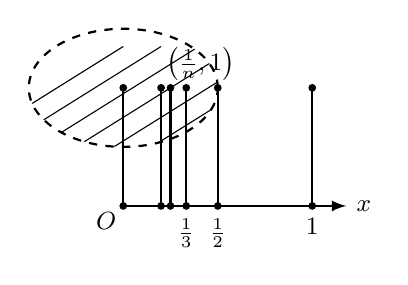
\begin{tikzpicture}[>=latex, x=2.4cm, y=1.5cm]
    % ---- 篦齿: x = 0, 1/5, 1/4, 1/3, 1/2, 1 ----
    \foreach \x in {0, 0.2, 0.25, 0.3333, 0.5, 1}{
      \draw[thick] (\x, 0) -- (\x, 1);
      \fill (\x, 1) circle (1.4pt);
      \fill (\x, 0) circle (1.4pt);
    }
    % ---- x 轴 ----
    \draw[->, thick] (0, 0) -- (1.18, 0) node[right] {\small $x$};
    \node[below left=-1pt] at (0, 0) {\small $O$};
    \node[below=1pt] at (0.3333, 0) {\small $\frac{1}{3}$};
    \node[below=1pt] at (0.5, 0) {\small $\frac{1}{2}$};
    \node[below=1pt] at (1, 0) {\small $1$};
    % ---- 开球 B((0,1); 1/2): 虚线圆 + 斜线阴影 ----
    \begin{scope}
      \clip (0, 1) circle (0.5);
      \foreach \k in {-1.0, -0.8, ..., 0.8}{
        \draw[thin] (\k, 0.35) -- (\k + 1.0, 1.35);
      }
    \end{scope}
    \draw[dashed, thick] (0, 1) circle (0.5);
    \node[right=1pt] at (0.16, 1.20) {\small $\left(\frac{1}{n}, 1\right)$};
  \end{tikzpicture}
  \caption{}\label{fig:7.4.2}
\end{figure}

\begin{exblock}{练习题 7.4}
  \item 设 $(X, \rho_{1})$ 与 $(Y, \rho_{2})$ 均为度量空间, $f\colon X \to Y$ 为一致连续映射, 证明: $f$ 为连续映射.

  \item 设 $(X, \rho_{1})$ 与 $(Y, \rho_{2})$ 均为度量空间, $f\colon X \to Y$ 为映射, 如果 $\exists \alpha \in (0, 1)$, s. t.
  \[
    \rho_{2}(f(x'), f(x'')) \leqslant \alpha \rho_{1}(x', x''),\quad \forall x', x'' \in X,
  \]
  则称 $f$ 为一个压缩映射. 显然, 它满足 Lipschitz 条件, 也为一致连续映射, 当然是连续映射. 当 $(X, \rho)$ 为完备度量空间, $f\colon X \to X$ 为压缩映射时, 令 $x_{n+1} = f(x_{n})$, 证明:
  \begin{enumerate}
    \item $\{x_{n}\}$ 为 $(X, \rho)$ 中的 Cauchy (基本) 点列, 记 $x_{0} = \lim\limits_{n \to +\infty} x_{n}$. 则 $f(x_{0}) = x_{0}$, 即 $x_{0}$ 为 $f$ 的一个不动点;
    \item $f$ 有惟一的一个不动点, 即 $\exists_{1}\xi \in X$, s. t. $f(\xi) = \xi$.
  \end{enumerate}

  \item 设 $A \subset \mathbb{R}^{n}$ 为非空集合, 证明: 点 $x$ 到 $A$ 的距离
  \[
    f_{A}(x) = \rho(x, A) = \inf_{y \in A} \rho(x, y)
  \]
  为 $\mathbb{R}^{n}$ 上的一致连续函数.
\end{exblock}

\begin{exblock}{思考题 7.4}
  \item 设 $\varphi\colon S^{n} \to S^{n}$ 为一个同胚, 满足: $\forall x \in S^{n}$, 有 $\varphi(\varphi(x)) = x$, 其中 $n \in \mathbb{Z}_{+}$. 证明: 对任何连续映射 $f\colon S^{n} \to \mathbb{R}$, $\exists \xi \in S^{n}$, s. t. $f(\xi) = f(\varphi(\xi))$. 当 $\varphi(x) = -x$ 时, 它就是\cref{ex:7.4.1}.

  \item 设 $(\mathbb{R}^{n}, \mathcal{T}_{\rho_{0}^{n}})$ 为 $n$ 维 Euclid 空间, $f\colon \mathbb{R}^{n} \to \mathbb{R}^{1}$ 为连续映射. 证明: 在 $\mathbb{R}^{1}$ 中最多存在两个点, 它在 $f$ 下的原像为非空的至多可数集.

  \item 设 $\boldsymbol{A} = (a_{ij})$ 为 $n \times n$ 的实方阵, 将它视为 $\mathbb{R}^{n^{2}}$ 中一个点 $(a_{11}, a_{12}, \cdots,\allowbreak a_{1n}, a_{21}, a_{22}, \cdots,\allowbreak a_{2n}, \cdots,\allowbreak a_{n1}, a_{n2}, \cdots, a_{nn})$. 于是, 将 $\{A = (a_{ij}) \mid a_{ij} \in \mathbb{R}\}$ 视为 $n^{2}$ 维 Euclid 空间 $(\mathbb{R}^{n^{2}}, \mathcal{T}_{\rho_{0}}^{n^{2}})$. 考虑 $n$ 阶正交群
  \[
    \boldsymbol{O}(n) = \boldsymbol{O}(n, \mathbb{R}) = \{\boldsymbol{P} \mid \boldsymbol{P}\boldsymbol{P}' = \boldsymbol{P}'\boldsymbol{P} = \boldsymbol{I},\ \boldsymbol{P} \text{ 为 } n \times n \text{ 实矩阵}\},
  \]
  其中 $\boldsymbol{I}$ 为单位矩阵, $P$ 为 $n \times n$ 实矩阵. 满足 $PP' = P'P = I$ 的实矩阵 $P$ 称为 $n$ 阶 (实) 正交矩阵. 显然, 有 $(\det P)^{2} = \det P \det P' = \det PP' = \det I = 1$, $\det P = \pm 1$. 证明:
  \begin{enumerate}
    \item $O(n)$ 为 $\mathbb{R}^{n^{2}}$ 中的有界闭集, 即为紧致集;
    \item $O^{+}(n) = O^{+}(n, \mathbb{R}) = \{P \mid PP' = P'P = I, \det P = 1\}$ 与 $O^{-}(n) = O^{-}(n, \mathbb{R}) = \{P \mid PP' = P'P = I, \det P = -1\}$ 都是道路连通的;
    \item $O(n)$ 不是道路连通的.
  \end{enumerate}

  \item 设 $\mathrm{GL}(n, \mathbb{R}) = \{A = (a_{ij}) \mid \det A \neq 0,\ A \text{ 为 } n \times n \text{ 实矩阵}\}$, 称它为 $n$ 阶一般线性群. 证明:
  \begin{enumerate}
    \item $\mathrm{GL}(n, \mathbb{R})$ 非紧致;
    \item $\mathrm{GL}^{+}(n, \mathbb{R}) = \{A \mid \det A > 0,\ A \text{ 为 } n \times n \text{ 实矩阵}\}$ 与 $\mathrm{GL}^{-}(n, \mathbb{R}) = \{A \mid \det A < 0,\ A \text{ 为 } n \times n \text{ 实矩阵}\}$ 都是道路连通的;
    \item $\mathrm{GL}(n; \mathbb{R})$ 不是道路连通的.
  \end{enumerate}
\end{exblock}
